\chapter{The Standard Model}

\subsection{Overview}

\todo{cite Yuval's lectures and notes somehow}

The Standard Model is another name for the theory of the internal symmetry group $SU(3)_C \otimes SU(2)_L \otimes U(1)_Y$ \todo{CHECK}.
This quantum field theory is the culmination of years of work in both theoretical and particle physics.  \todo{cite}
In this thesis, we take the view one constructs a model with the field content and symmetries as inputs, and then writes down the most general Lagrangian consistent with those symmetries.
This will be applicable for this chapter and the following one.
Additional theoretical background is in \ref{app:qft_symmetries}.

\subsection{Field Content}

The Standard Model field content is
\begin{equation}
\begin{aligned}
\text{Fermions } Q_L(3,2)_{+1/3}, \xspace  U_R(3,1)_{+4/3},\xspace  D_R(3,1)_{-2/3} ,\xspace  L_L(1,2)_{-1} ,\xspace  E_R(1,1)_{-2}\\
\text{Scalar (Higgs) } \xspace \phi(1,2)_{+1} \\
\text{Vector Fields } \xspace G^\mu(8,1)_0 \xspace W^\mu(1,3)_0  \xspace B^\mu(1,1)_0
\end{aligned}
\end{equation}
where the $(A, B)_Y$ notation represents the irreducible representation under $SU(3)$ and $SU(2)$, with $Y$ being the electroweak hypercharge.
Each of these fields has an additional index, representing the three generation of fermions.

We observed that $Q_L, U_R,$ and $D_R$ are triplets under $SU(3)_C$; these are the \textit{quark} fields.
The \textit{color} group, $SU(3)_C$ is mediated by the \textit{gluon} field $G^\mu(8,1)_0$, which has 8 degrees of freedom.
The fermion fields $L_L(1,2)_{-1}$ and $  E_R(1,1)_{-2} $ are singlets under $SU(3)_C$; we call them the \textit{lepton} fields.

Next, we note the ``left-handed'' (``right-handed'') fermion fields, denoted by $L$ ($R$) subscript,
The left-handed fields form doublets under $SU(2)_L$.
These are mediated by the three degrees of freedom of the  ``W'' fields $W^\mu(1,3)_0$.
These fields only act on the left-handed particles of the Standard Model.
This is the reflection of the ``chirality'' of the Standard Model; the left-handed and right-handed particles are treated differently by the electroweak forces.
The right-handed fields, $U_R, D_R$, and $E_R$, are singlets under $SU(2)_L$.

The $U(1)_Y$ symmetry is associated to the $B^\mu(1,1)_0$ boson with one degree of freedom.
The charge $Y$ is known as the electroweak hypercharge.

To better understand the phenomenology of the Standard Model, let us investigate each of the \textit{sectors} of the Standard Model separately.

\subsection{Electroweak sector}

The electroweak sector refers to the $SU(2)_L \otimes U(1)_Y$ portion of the Standard Model gauge group.
Following our philosophy of writing all gauge-invariant and renormalizable ( maximum degree 4 in the mass) terms, the electroweak Lagrangian can be written as
\begin{equation}
\Lagr =  W^{\mu\nu}_a W_{\mu\nu}^a + B^{\mu\nu} B_{\mu\nu} + (\Dmuup \phi)^\dagger \Dmu \phi -  \mu^2 \phi^\dagger \phi - \lambda (\phi^\dagger \phi)^2.
\end{equation}
where $W^{\mu\nu}_a$ are the three ($a=1,2,3$) gauge bosons associated to the $SU(2)_L$ gauge group, $B^{\mu\nu}$ is the one gauge boson of the $U(1)_Y$ gauge group, and $\phi$ is the complex Higgs multiplet with weak hypercharge $Y = 1$.
The covariant derivative $\Dmuup$ is given by
\begin{equation}
\Dmuup = \dmuup  + i \frac{g}{2} W^\mu_a \sigma_a + \frac{i}{2} g' B^\mu
\end{equation}
where $\sigma_a$ are the Pauli matrices, which are the generators for $SU(2)_L$, and $g$ and $g'$ are the $SU(2)_L$ and $U(1)_Y$ coupling constants, respectively.
The field strength tensors  $W^{\mu\nu}_a$ and $B^{\mu\nu}$ are given by the commutator of the covariant derivative associated to each field
\begin{equation} \label{eq:ew_field_strength_tensor}
\begin{aligned}
B^{\mu\nu}   = \dmuup B^\nu - \partial^\nu B^\mu \\
W^{\mu\nu}_a = \dmuup W^\nu_a - \partial^\nu W^\mu_a - g \epsilon_{abc} W^\mu_a W^\nu_b, i = 1,2,3
\end{aligned}
\end{equation}

The terms proportional in the Lagrangian to $\mu^2$ and $\lambda$ make up the ``Higgs potential'' \todo{Cite}.
As normal (i.e. in Appendix \ref{app:qft_symmetries}), we restrict $\lambda > 0$ to guarantee our potential is bounded from below, and we also require $\mu^2 < 0$, which gives us the standard ``sombrero'' potential shown in \ref{fig:sombrero}. \todo{footnote how we probably shouldn't say mexican hat?}

\todo{CITE THIS PICTURE}
\begin{figure} \label{fig:sombrero}
\caption{Sombrero potential}
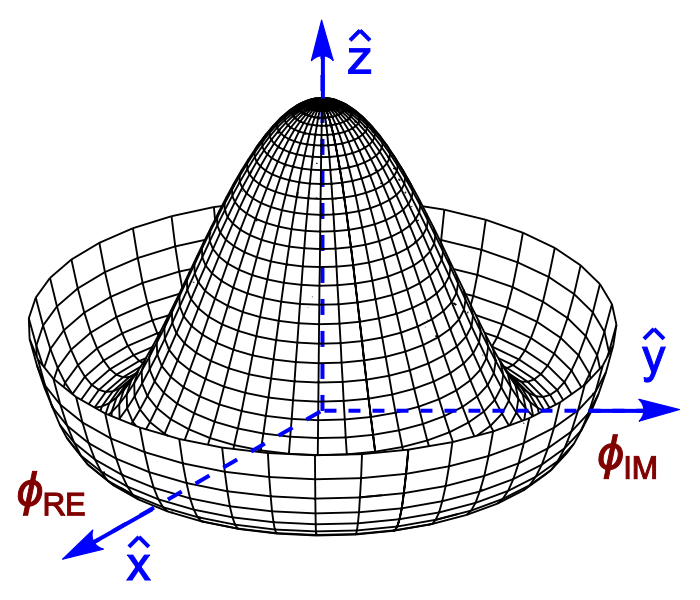
\includegraphics[width=\linewidth]{sombrero_potential}
\end{figure}

This potential has a minimum at $VALUE$; the ground state is \textit{spontaneously} broken by the choice of ground state, which induces a vacuum expection value (VEV).
Without loss of generality, we can choose the Higgs field $\phi$ to point in the real direction, and write the Higgs field $\phi$ in the following form :
\begin{equation}
\phi = \frac{1}{\sqrt{2}} \exp( \frac{i}{v} \sigma_a \theta_a ) \begin{pmatrix} 0 \\ v + h(x) \end{pmatrix}.
\end{equation}
We can choose a gauge to rotate away the dependent on $\theta_a$, such that we can write simply
\begin{equation}
\label{eq:higgs_field_after_ssb}
\phi = \frac{1}{\sqrt{2}} \begin{pmatrix} 0 \\ v + h(x) \end{pmatrix}.
\end{equation}
Now, we can see how the masses of the vector bosons are generated from the application of the Higgs mechanism.
We plug Eq.\ref{eq:higgs_field_after_ssb} back into the electroweak Lagrangian, and only showing the relevant mass terms in the vacuum state where $h(x) = 0$  see that (dropping the Lorentz indices) :
\begin{equation}
\begin{aligned}
\Lagr_M = \frac{1}{8} |\begin{pmatrix} gW_3 + g'B & g(W_1 - iW_2) \\ g(W_1 + iW_2) & -gW_3 + g'B \end{pmatrix}  \begin{pmatrix} 0 \\ v \end{pmatrix} |^2\\ = \frac{g^2 v^2}{8}[W_1^2 + W_2^2 + (\frac{g'}{g}B - W_3)^2]
\end{aligned}
\end{equation}\todo{CHECK THIS EQUATION, especially the squaring?, I'm a bit confused here}

Defining the \textit{Weinberg} angle $\tan(\theta_W) = g'/g$ and the following physical fields :
\begin{equation}
\begin{aligned}
W^{\pm} = \frac{1}{\sqrt{2}}(W_1 \mp iW_2) \\
Z^0 = \cos \theta_W W_3 - \sin\theta_W B \\
A^0 = \sin \theta_W W_3 + \cos\theta_W B
\end{aligned}
\end{equation}
we see we can write the piece of the Lagrangian associated to the vector boson masses as
\begin{equation}
\Lagr_{M_V} = \frac{1}{4} g^2 v^2 W^+ W^- + \frac{1}{8} (g^2 + g'^2)v^2 Z^0 Z^0 .
\end{equation}
and we have the following values of the masses for the vector bosons :
\begin{equation}
\begin{aligned}
m_W^2 = \frac{1}{4}  v^2 g^2 \\
m_Z^2 = \frac{1}{4}  v^2 (g^2 + g'^2) \\
m_A^2 = 0
\end{aligned}
\end{equation}
We thus see how the Higgs mechnanism gives rise to the masses of the $W^{\pm}$ and $Z$ boson in the Standard Model; the mass of the photon is zero, as expected.
The $SU(2)_L \otimes U(1)_Y$ symmetry of the initially massless $W_{1,2,3}$ and $B$ fields is broken to the $U(1)_{EM}$.
Of the four degrees of freedom in the complex Higgs doublet, three are ``eaten'' when we give mass to the $W^\pm$ and $Z_0$, while the other degree of freedom is the Higgs particle, as found in 2012 \todo{cite}.
% \subsection{$\Lagr_{kin}$}

\subsection{Quantum Chromodynamics}

Quantum chromodynamics (or the theory of the \textit{strong} force) characterizes the behavior of \textit{colored} particles, collectively known as \textit{partons}.
The partons of the Standard Model are the (fermionic) quarks, and the (bosonic) gluons.
The strong force is governed by $SU(3)_C$ which is an unbroken symmetry in the Standard Model; this implies the gluon remains massless.
Defining the covariant derivative for QCD as
\begin{equation}
\Dmuup = \dmuup + ig_s G^\mu_a L_a
\end{equation}
where $L_a$ are the generators of $SU(3)_C$, often represented by the Gell-Mann matrices, and $g_s$ is the coupling constant of the strong force. \todo{check the logic here? are tehy actually them?}.
The QCD Lagrangian then is given by
\begin{equation}
\Lagr_{\text{QCD}} = i \bar{\psi}_f \Dmu \gamma^\mu \psi_f - \frac{1}{4} G^a_{\mu\nu} G_a^{\mu\nu}
\end{equation}
where the summation over $f$ is for quarks \textit{families}, and $ G_a^{\mu\nu}$ is the gluon field strength tensor, given by
\begin{equation}
G^{\mu\nu}_a = \dmuup G^\nu_a - \partial^\nu G^\mu_a - g_s f^{abc} G^\mu_b G^\nu_c, a = 1,...,8
\end{equation}
where $f^{abc}$ are the structure constants of $SU(3)_C$, which are analogus \todo{sp} to $\epsilon_{abc}$ for $SU(2)_L$.
The kinetic term for the quarks is contained in the standard $\dmu$ term, while the field strength term contains the interactions between the quarks and gluons, as well as the gluon self-interactions.

Written down in this simple form, the QCD Lagrangian does not seem much different from the QED Lagrangian, with the proper adjustments for the different group structures.\todo{maybe cite the QED lagrangian?}
The gluon is massless, like the photon, so one could n\"aively expect an infinite range force, and it pays to understand why this is not the case.
The reason for this fundamental difference is the gluon self-interactions  \todo{reference figure} arising in the field strength tensor term of the Lagrangian.
This leads to the phenomena of \textit{color confinement}, which describes how one only observes color-neutral particles alone in nature.
In contrast to the electromagnetic force, particles which interact via the strong force experience a \textit{greater} force as the distance between the particles increases.
At long distances, the potential is given by $V(r) = -kr$.
At some point, it is more energetically favorable to create additional partons out of the vacuum than continue pulling apart the existing partons, and the colored particles undergo \textit{fragmentation}.
This leads to \textit{hadronization}.
Bare quarks and gluons are actually observed as sprays of hadrons (primarly kaons and pions); these sprays are known as \textit{jets}, which are what are observed by experiments.

It is important to recognize the importance of understanding these QCD interactions in high-energy hadron colliders such as the LHC.
Since protons are hadrons, proton-proton collisions such as those produced by the LHC are primarily governed by the processes of QCD.
In particular, by far the most frequent process observed in LHC experiments is dijet production from gluon-gluon interactions.
These gluons that interact are part of the \textit{sea} particles inside the proton; the simple $p = uud$ model does not apply.
The main \textit{valence} $uud$ quarks are constantly interacting via gluons, which can themselves radiate gluons or split into quarks, and so on.
A more useful understanding is given by the colloquially-known \textit{bag} model, where the proton is seen as a ``bag'' of (in principle) infinitely many partons, each with energy $ E < \sqrt{s} = 6.5 \TeV$.
\todo{get that cross section picture}.
\todo{bag model?}.
One then collides this (proton) bag with another, and views the products of this very complicated collision.

Fortunately, we are generally saved by the QCD factorization theorem \todo{cite QCD factorization}.
This allows one to understand the hard (i.e. short distance or highest energy) $2 \rightarrow 2$ parton process using the tools of perturbative QCD, while making series of approximations known as a \textit{parton shower} model to understand the additional corrections from nonpertubative QCD.
We will discuss the reconstruction of jets by experiments in Ch.\ref{Chapter-ATLAS}.

\todo{show ratio of ee to qq?}.

\subsection{Fermions}

\todo{CITE THIS PICTURE}
\begin{figure}\label{fig:sm_interactions}
\caption{The interactions of the Standard Model}
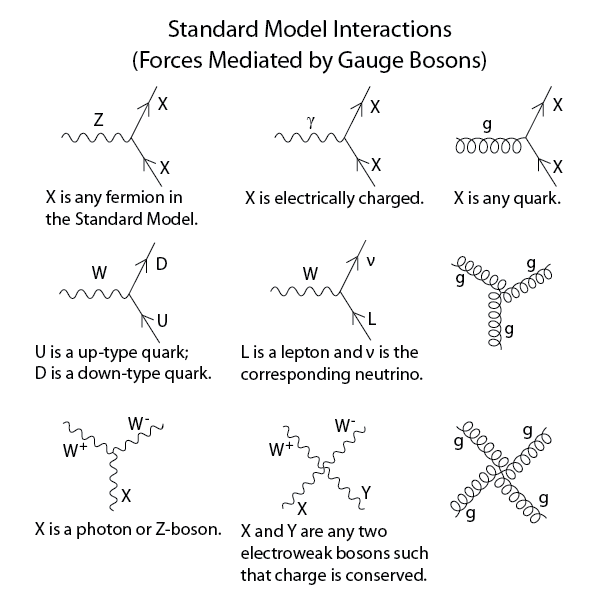
\includegraphics[width=\linewidth]{Standard_Model_Feynman_Diagram_Vertices}
\end{figure}

We will now look at the fermions, and summarize their interactions.

As noted earlier with regards to the field content, the fermions of the Standard Model can be first distinguished between those that interact via the strong force (quarks) and those which do not (leptons).

There are six leptons in the Standard Model, which can be placed into three \textit{generations}. \todo{cite pdg probably}
There is the electron ($e)$, muon ($\mu$), and tau ($\tau$), each of which has an associated neutrino ($\nu_e, \nu_\mu, \nu_\tau$).
Each of the ``electron-like'' leptons has electromagnetic charge $-1$, while the neutrinos all have $q_{EM} = 0$.

Often in an experimental context, lepton is used to denote the electron (stable) and muon (metastable), due to their striking experimental signatures.
Taus are often treated separately, due to their much shorter lifetime of $\tau_{\tau}  $; these decay through hadrons or the other leptons, so often physics analyses at the LHC treat them as jets or leptons, as will be done in this thesis.

As the neutrinos are electrically neutral, nearly massless, and only interact via the weak force, it is quite difficult to observe them directly.\todo{footnote?}
Since LHC experiments rely overwhelmingly on electromagnetic interactions to observe particles, the presence of neutrinos is not observed directly.
Neutrinos are instead observed by the conservation of four-momentum in the plane transverse to the proton-proton collisions, known as \textit{missing transverse energy}.

There are six quarks in the Standard Model : up, down, charm, strange, top, and bottom. Quarks are similar organized into three generations :
\begin{equation}
\begin{pmatrix} u & d \end{pmatrix} , \begin{pmatrix} c & s \end{pmatrix}, \begin{pmatrix} t & b \end{pmatrix}
\end{equation}
where we speak of ``up-like'' quarks and ``down-like'' quarks.

Each up-like quark has charge $q_{up} = 2/3$, while the down-like quarks have $q_{down} = -1/3$.
At the high energies of the LHC, one often makes the distinction between the light quarks ($u,d,c,s$), the bottom quark, and top quark.
In general, due to the hadronization process described above, the light quarks are indistinguishable by LHC experiments, and reconstructed as jets.\todo{footnote about charm tagging}.
The bottom quark hadronizes primarly through a relatively long-lived particle known as the $ B$ (name), which generally travels a short distance before decay.
This feature allows what is known as \textit{b-tagging}; this will be further discussed in Ch.\todo{refCh ATLAS.}
Due to its large mass, the top quark decays before it can hadronize; there are no bound states associated to the top quark.
The top is of particular interest at the LHC, due to its large mass

An overview of all the interactions in the Standard Model can be found in \ref{fig:sm_interactions}.


\section{Deficiencies of the Standard Model}

By using the asterisk to start a new section, I keep the section from appearing in the table of contents.
If you want your sections to be numbered and to appear in the table of contents, remove the asterisk.



% \subsection{$\Lagr_{\psi}$ }

% We cannot write down any mass terms for fermions in the Standard Model.
% Dirac mass terms are forbidden since they are all assigned to ``chiral'' representations of the gauge symmetry.
% Majorana mass terms are disallowed since there are no fields with $Y \slashed{=} 0$.

% \subsection{$\Lagr_{Yuk}$ }

% We write the Yukawa portion of the Standard Model Lagrangian

% \begin{equation}
% \Lagr_{Yuk} = Y_{ij}\bar{L_{Li} E_{Rj}} \phi + h.c.
% \end{equation}

% The Yukawa matrix $Y$ is a general complex 3 $\times$ 3 matrix of dimensionless couplings which can be diagonalized, leading to a diagonal matrix with only three real parameters $(y_e , y_\mu , y_\tau)$.
% This reflects the fact that for the electron, muon, and tau lepton, the interaction basis is the same as the mass basis; this is the same as saying an electron has a well-defined mass.

% \section{$\Lagr_\phi$, Electroweak Symmetry breaking and the Higgs Boson}

% Let us now recall that local gauge invariance means that the vector fields in this theory are \textit{massless}.
% N\"aively, it seems this combined with the chirality of the Standard Model, that \textit{none} of the fields have masses.
% The solution to this seeming conundrum is of course the well-known ``Higgs'' mechanism, described in Sec. \ref{subsec:symmetry_breaking}.

% In the Standard Model, the Higgs potential is given by
% \begin{equation} \label{eq:higgs_potential}
% \Lagr_\phi = -\mu^2 \phi^\dagger \phi - \lambda (\phi^\dagger \phi)^2.
% \end{equation}

% Since $\lambda$ is dimensionless and real, to have a potential bounded from below, we require $\lambda > 0$.
% To break the gauge symmetry, we require $\mu^2 < 0$, leading again to the sombrero potential \ref{fig:sombrero}.
% We define
% \begin{equation}
% v^2 = - \frac{\mu^2}{\lambda}.
% \end{equation}

% This allows us to write \ref{eq:higgs_potential} as
% \begin{equation} \label{eq:higgs_potential_rewritten}
% \Lagr_\phi = - \lambda (\phi^\dagger \phi - \frac{v^2}{2})^2
% \end{equation}
% after dropping the constant term.

% This means the $\phi$ field acquires a VEV $|<\phi>| = v/\sqrt{2}$.
% Choosing the convenient gauge
% \begin{equation}
% \phi = \begin{pmatrix} 0 \\ v/\sqrt{2} \end{pmatrix},
% \end{equation}

% The VEV breaks the $SU(2)_L \otimes U(1)_Y$ symmetry to a $U(1)_{EM}$ subgroup.
% We can identify the unbroken generator of this $U(1)_{EM}$ subgroup as $Q_{EM} = T_3 + Y/2$, since this vanishes in the down component
% \begin{equation}
% Q_{\gamma} \phi = (T_3 + Y/2) \phi = (\frac{1}{2} \sigmathree + \frac{1}{2} I ) \begin{pmatrix} 0 \\ v/\sqrt{2} \end{pmatrix}.
% \end{equation}
% Here we see the indicative $\gamma$ for the photon, as this unbroken $U(1)_{EM}$ symmetry is of course the symmetry associated to the electromagnetic force mediated by the gauge boson known as the photon.

% There are three broken generators : $T_1, T_2, T_3 - Y/2$.
% These are each associated to one of the massive gauge bosons induced by the symmetry breaking.
% Choosing a gauge which rotates away the ``eaten'' Goldstone boson degrees of freedom, we can write the Higgs field as
% \begin{equation}
% \label{eq:higgs_field}
% \phi = \frac{1}{\sqrt{2}}\begin{pmatrix} 0 \\ v + h(x) \end{pmatrix}.
% \end{equation}

% \section{Particle Spectrum : Standard Model Lagrangian after Electroweak Symmetry Breaking}

% We can now return to the Standard Model Lagrangian and use the equation for the Higgs field after EWSB \ref{eq:higgs_field}.
% This will show us the ``physical'' particle content of the Standard Model.

% \subsection{Particle content associated to $\Lagr_\phi$}

% Setting $phi$ as in Eq.\ref{eq:higgs_field}, we quickly see that we can rewrite Eq.\ref{eq:higgs_potential_rewritten} as
% \todo{ CHECK FACTORS OF TWO}
% \begin{equation}
% \Lagr_\phi = - \lambda (\phi^\dagger \phi - \frac{v^2}{2})^2  = - \lambda ( \frac{1}{2} (v + h(x))^2 - \frac{v^2}{2})^2 = - \lambda ( h(x)^2 + vh(x))^2 = -\lambda ( h(x)^4 + v h(x)^3 + \frac{v^2}{2} h(x)^2 ).
% \end{equation}

% Interpreting the Higgs field squared term as the mass term of the Higgs boson, we see that $m_H = \sqrt{2 \lambda} v$.

% \subsection{Particle content associated to $\Lagr_{kin}$}

% Again using Eq.\ref{eq:higgs_field} and $\Dmuup = \dmuup + ig_s G^\mu_a L_a + i g W^\mu_a T_a + i g' Y B^\mu $, we can see how the mass terms associated to the three massive gauge bosons, and also see how the photon stays massless.
% The mass terms for the gauge boson fields come from the kinetic term of the Higgs field :
% For each of the vector boson fields, we have the follow field strengths :

% \begin{equation}
% \begin{aligned}
% G^{\mu\nu}_a = \dmuup G^\nu_a + \partial^\nu G^\mu_a - g_s f_{abc} G^\mu_b G^\nu_c \\
% W^{\mu\nu}_a = \dmuup W^\nu_a + \partial^\nu W^\mu_a - g \epsilon_{abc} W_b^\mu W_c^\nu \\
% B^{\mu\nu}   = \dmuup B^\nu   + \partial^\nu B^\mu
% \end{aligned}
% \end{equation}

% where $g$ and $g_s$ are the electroweak and strong coupling constant.

% We can write the covariant derivative for the Standard Model as
% \begin{equation}
% \Dmuup = \dmuup + ig_s G^\mu_a L_a + i g W^\mu_a T_a + i g' Y B^\mu
% \end{equation}
% where $L_a$ and $T_a$ are the generators of $SU(3)_C $ and $SU(2)_L$ respectively for each of the representations.
% Explicitly, for the $SU(3)_C$ triplets, $L_a = \frac{1}{2} \lambda_a$ and for the $SU(3)_C$ singlets, $L_a = 0$. \todo{GELLMANN and Pauli matrices}.
% For $SU(2)_L$ doublets, $T_a = \frac{1}{2} \sigma_a $ and for $SU(2)_L$ singlets, $T_a = 0$.

% The combination of these terms allows us to write the kinetic terms of the Lagrangian as
% \begin{equation}
% \begin{aligned}
% \Lagr_{kin} = G^{\mu\nu} G_{\mu\nu} + W^{\mu\nu} W_{\mu\nu} + B^{\mu\nu} B_{\mu\nu}\\
%  + \Dmuup Q_L \Dmu Q_L + \Dmuup U_R \Dmu U_R +  \Dmuup D_R \Dmu D_R + \Dmuup L_L \Dmu L_LL + \Dmuup E_R \Dmu E_R
% \end{aligned}
% \end{equation}
